% !TEX TS-program = pdflatex
\documentclass[11pt]{article}

% -------------------- Packages --------------------
\usepackage[a4paper,margin=1in]{geometry}
\usepackage{amsmath,amssymb}
\usepackage[T1]{fontenc}
\usepackage{lmodern}
\usepackage{xcolor}
\usepackage{tcolorbox}
\tcbuselibrary{skins,breakable}
\usepackage{enumitem}
\usepackage{hyperref}
\usepackage{tikz}
\usetikzlibrary{calc,patterns}

\pagestyle{empty}

% -------------------- Dark Theme Colors --------------------
\definecolor{bg}{HTML}{000000}
\definecolor{pairbg}{HTML}{121212}
\definecolor{solbg}{HTML}{0A0A0A}
\definecolor{border}{HTML}{2A2A2A}
\definecolor{text}{HTML}{FFFFFF}
\definecolor{muted}{HTML}{C9CDD3}
\definecolor{gold}{HTML}{FFD700}
\definecolor{green}{HTML}{4ADE80}
\definecolor{cyan}{HTML}{38BDF8}

\pagecolor{bg}
\color{text}

\hypersetup{
  colorlinks=true,
  linkcolor=cyan,
  urlcolor=cyan
}

\setlength{\parindent}{0pt}
\setlength{\parskip}{10pt}

\setlist[itemize]{left=1.4em,itemsep=6pt,topsep=6pt}
\setlist[enumerate]{left=1.6em,itemsep=4pt,topsep=4pt}

% -------------------- tcolorbox Base --------------------
\tcbset{
  enhanced,
  breakable,
  arc=12pt,
  boxrule=0.8pt,
  left=16pt,right=16pt,top=12pt,bottom=12pt
}

\newtcolorbox{QAPair}[1]{%
  colback=pairbg,
  colbacklower=solbg,
  colframe=border,
  coltext=text,
  title=\textcolor{gold}{\bfseries #1},
  fonttitle=\bfseries,
  coltitle=text,
  segmentation style={draw=border, dashed, line width=0.6pt},
}

\newtcolorbox{QuickBox}{%
  colback=pairbg,
  colframe=cyan,
  coltext=text,
  fontupper=\color{text},
  borderline north={4pt}{0pt}{cyan},
  arc=14pt,
  boxrule=0.8pt
}

% Helper for step headings
\newcommand{\Step}[1]{\textcolor{muted}{\textbf{Step #1:}}}

% -------------------- TikZ Styles --------------------
\tikzset{
  vennCircle/.style={draw=muted, line width=0.9pt},
  vennFill/.style={fill=cyan, fill opacity=0.22},
  vennLabel/.style={text=text, font=\small},
  vennText/.style={text=text, font=\small},
  axis/.style={->, draw=muted, line width=0.8pt},
  seg/.style={draw=cyan, line width=0.95pt},
  dseg/.style={draw=muted, dashed, line width=0.75pt},
  pt/.style={circle, fill=cyan, inner sep=1.6pt},
  ptlab/.style={text=text, font=\small}
}

% ============================================================
\begin{document}

\begin{center}
{\LARGE\bfseries \textcolor{gold}{Miscellaneous Exercise 7 --- Solutions}}\\[-2pt]
\end{center}

\begin{QuickBox}
{\color{cyan}\bfseries Quick formulas (Coordinate Geometry)}\par\medskip
\begin{itemize}
\item \textbf{Distance between two points:} If $P(x_1,y_1)$, $Q(x_2,y_2)$ then
\[
PQ=\sqrt{(x_2-x_1)^2+(y_2-y_1)^2}.
\]
\item \textbf{Midpoint:} Midpoint of $P(x_1,y_1)$ and $Q(x_2,y_2)$ is
\[
M\Big(\frac{x_1+x_2}{2},\frac{y_1+y_2}{2}\Big).
\]
(On a number line: midpoint of $a,b$ is $\frac{a+b}{2}$.)
\item \textbf{Distance from axes:} For $(x,y)$, distance from $x$-axis is $|y|$, from $y$-axis is $|x|$.
\item \textbf{Quadrant signs:}
I $(+,+)$,\; II $(-,+)$,\; III $(-,-)$,\; IV $(+,-)$.
\item \textbf{Circle center from diameter endpoints:} Center is the midpoint of the diameter endpoints.
\item \textbf{Parallelogram test:} A quadrilateral is a parallelogram if both pairs of opposite sides are parallel (equal slopes), or if diagonals bisect each other.
\item \textbf{Rhombus test (easy):} If all four sides of a quadrilateral are equal, it is a rhombus (and it is also a parallelogram).
\end{itemize}
\end{QuickBox}

% ============================================================
% Q1 (MCQs)
% ============================================================

\begin{QAPair}{Question 1 (i) --- MCQ}
\textcolor{gold}{\bfseries Question:} If $A\left(\frac32,-\frac74\right)$, $B\left(3,\frac34\right)$, $C(3,-2)$ and $D\left(1,\frac12\right)$, then relationship between distances $AB$ and $CD$ is:\par
\begin{itemize}
\item[(a)] $AB>CD$
\item[(b)] $AB<CD$
\item[(c)] $AB=CD$
\item[(d)] $AB=\frac12\,CD$
\end{itemize}
\tcblower
\textcolor{green}{\bfseries Answer:} \textbf{(b)}\par
\[
\begin{aligned}
\Step{1}\;& AB=\sqrt{\Big(3-\frac32\Big)^2+\Big(\frac34-(-\frac74)\Big)^2}
=\sqrt{\Big(\frac32\Big)^2+\Big(\frac{10}{4}\Big)^2}
=\sqrt{\frac94+\frac{25}{4}}=\sqrt{\frac{34}{4}}=\frac{\sqrt{34}}{2}.\\[4pt]
\Step{2}\;& CD=\sqrt{(1-3)^2+\Big(\frac12-(-2)\Big)^2}
=\sqrt{(-2)^2+\Big(\frac52\Big)^2}
=\sqrt{4+\frac{25}{4}}=\sqrt{\frac{41}{4}}=\frac{\sqrt{41}}{2}.\\[4pt]
\Step{3}\;& \sqrt{34}<\sqrt{41}\Rightarrow AB<CD \Rightarrow \text{(b).}
\end{aligned}
\]
\end{QAPair}

\begin{QAPair}{Question 1 (ii) --- MCQ}
\textcolor{gold}{\bfseries Question:} If $a$ and $b$ are any two points on a coordinate line (number line), then its midpoint will be:\par
\begin{itemize}
\item[(a)] $\dfrac{a+b}{2}$
\item[(b)] $\left(\dfrac{a}{2},\dfrac{b}{2}\right)$
\item[(c)] $\left(\dfrac{a}{2},b\right)$
\item[(d)] $\left(a,\dfrac{b}{2}\right)$
\end{itemize}
\tcblower
\textcolor{green}{\bfseries Answer:} \textbf{(a)}\par
\[
\begin{aligned}
\Step{1}\;& \text{On a number line, midpoint is the average.}\\
\Step{2}\;& \Rightarrow M=\dfrac{a+b}{2}\ \Rightarrow \text{(a).}
\end{aligned}
\]
\end{QAPair}

\begin{QAPair}{Question 1 (iii) --- MCQ}
\textcolor{gold}{\bfseries Question:} $(5,2)$, $(7,0)$, $(1,-2)$ and $(-1,0)$ are the vertices of a:\par
\begin{itemize}
\item[(a)] parallelogram
\item[(b)] square
\item[(c)] trapezium
\item[(d)] kite
\end{itemize}
\tcblower
\textcolor{green}{\bfseries Answer:} \textbf{(a)}\par
\[
\begin{aligned}
\Step{1}\;& \text{Take the points in order }A(5,2),B(7,0),C(1,-2),D(-1,0).\\
\Step{2}\;& m_{AB}=\frac{0-2}{7-5}=-1,\qquad
m_{CD}=\frac{0-(-2)}{-1-1}=\frac{2}{-2}=-1 \Rightarrow AB\parallel CD.\\
\Step{3}\;& m_{BC}=\frac{-2-0}{1-7}=\frac{-2}{-6}=\frac13,\qquad
m_{DA}=\frac{2-0}{5-(-1)}=\frac{2}{6}=\frac13 \Rightarrow BC\parallel AD.\\
\Step{4}\;& \text{Both pairs of opposite sides are parallel } \Rightarrow \text{parallelogram } \Rightarrow \text{(a).}
\end{aligned}
\]
\end{QAPair}

\begin{QAPair}{Question 1 (iv) --- MCQ}
\textcolor{gold}{\bfseries Question:} The triangle with vertices $(1,-3)$, $(3,2)$ and $(-2,4)$ is:\par
\begin{itemize}
\item[(a)] a right triangle
\item[(b)] an isosceles triangle
\item[(c)] a right isosceles triangle
\item[(d)] an equilateral triangle
\end{itemize}
\tcblower
\textcolor{green}{\bfseries Answer:} \textbf{(c)}\par
\[
\begin{aligned}
\Step{1}\;& AB^2=(3-1)^2+(2-(-3))^2=2^2+5^2=29.\\
\Step{2}\;& BC^2=(-2-3)^2+(4-2)^2=(-5)^2+2^2=29.\\
\Step{3}\;& CA^2=(1-(-2))^2+(-3-4)^2=3^2+(-7)^2=58.\\
\Step{4}\;& AB^2=BC^2 \Rightarrow \text{isosceles, and } AB^2+BC^2=29+29=58=CA^2\\
&\Rightarrow \text{right angle (at }B\text{). So it is a right isosceles triangle } \Rightarrow \text{(c).}
\end{aligned}
\]
\end{QAPair}

\begin{QAPair}{Question 1 (v) --- MCQ}
\textcolor{gold}{\bfseries Question:} Mid-point of $(c,-d)$ and $(-d,c)$ is:\par
\begin{itemize}
\item[(a)] $\left(\dfrac{c}{2},-\dfrac{d}{2}\right)$
\item[(b)] $\left(\dfrac{-c-d}{2},\dfrac{-d-c}{2}\right)$
\item[(c)] $\left(\dfrac{-d+c}{2},\dfrac{c-d}{2}\right)$
\item[(d)] $(c-d,-d+c)$
\end{itemize}
\tcblower
\textcolor{green}{\bfseries Answer:} \textbf{(c)}\par
\[
\begin{aligned}
\Step{1}\;& M=\Big(\frac{c+(-d)}{2},\frac{-d+c}{2}\Big)
=\Big(\frac{c-d}{2},\frac{c-d}{2}\Big).\\
\Step{2}\;& \text{Option (c) gives exactly this (same expressions).}
\end{aligned}
\]
\end{QAPair}

\begin{QAPair}{Question 1 (vi) --- MCQ}
\textcolor{gold}{\bfseries Question:} If $P(2,3)$ is the midpoint of $A(x,4)$ and $B(-3,y)$, then the coordinates of $(x,y)$ are:\par
\begin{itemize}
\item[(a)] $\left(-\dfrac12,\dfrac{3+b}{2}\right)$
\item[(b)] $(5,-1)$
\item[(c)] $\left(\dfrac{x-3}{2},\dfrac{y+4}{2}\right)$
\item[(d)] $(7,2)$
\end{itemize}
\tcblower
\textcolor{green}{\bfseries Answer:} \textbf{(d)}\par
\[
\begin{aligned}
\Step{1}\;& \frac{x+(-3)}{2}=2 \Rightarrow x-3=4 \Rightarrow x=7.\\
\Step{2}\;& \frac{4+y}{2}=3 \Rightarrow 4+y=6 \Rightarrow y=2.\\
\Step{3}\;& (x,y)=(7,2)\Rightarrow \text{(d).}
\end{aligned}
\]
\end{QAPair}

\begin{QAPair}{Question 1 (vii) --- MCQ}
\textcolor{gold}{\bfseries Question:} If two ordered pairs $(4,5)$ and $\left(\dfrac{a+1}{2},\,b-3\right)$ are equal, then the value of $a$ is:\par
\begin{itemize}
\item[(a)] $4$
\item[(b)] $8$
\item[(c)] $7$
\item[(d)] $5$
\end{itemize}
\tcblower
\textcolor{green}{\bfseries Answer:} \textbf{(c)}\par
\[
\begin{aligned}
\Step{1}\;& \frac{a+1}{2}=4 \Rightarrow a+1=8 \Rightarrow a=7.\\
\Step{2}\;& \Rightarrow \text{(c).}
\end{aligned}
\]
\end{QAPair}

\begin{QAPair}{Question 1 (viii) --- MCQ}
\textcolor{gold}{\bfseries Question:} In which quadrant, the point $(-4,-(-6))$ lies?\par
\begin{itemize}
\item[(a)] first
\item[(b)] second
\item[(c)] third
\item[(d)] fourth
\end{itemize}
\tcblower
\textcolor{green}{\bfseries Answer:} \textbf{(b)}\par
\[
\begin{aligned}
\Step{1}\;& (-4,-(-6))=(-4,6).\\
\Step{2}\;& x<0,\ y>0 \Rightarrow \text{Quadrant II} \Rightarrow \text{(b).}
\end{aligned}
\]
\end{QAPair}

\begin{QAPair}{Question 1 (ix) --- MCQ}
\textcolor{gold}{\bfseries Question:} In the adjoining figure of a line: $d(A,C)-d(B,C)=$\par
\begin{itemize}
\item[(a)] $d(B,A)$
\item[(b)] $d(C,B)$
\item[(c)] $d(A,B)$
\item[(d)] both a \& c
\end{itemize}
\tcblower
\textcolor{green}{\bfseries Answer:} \textbf{(d)}\par
\[
\begin{aligned}
\Step{1}\;& \text{On a line with }A\text{---}B\text{---}C:\quad d(A,C)=d(A,B)+d(B,C).\\
\Step{2}\;& d(A,C)-d(B,C)=d(A,B).\\
\Step{3}\;& d(A,B)=d(B,A)\Rightarrow \text{both (a) and (c) are true } \Rightarrow \text{(d).}
\end{aligned}
\]
\par\medskip
\begin{center}

\begin{tikzpicture}[scale=1.0]
  \draw[muted, line width=0.9pt] (-4,0)--(4,0);
  \draw[muted, line width=0.9pt] (-2.5,-0.12)--(-2.5,0.12);
  \draw[muted, line width=0.9pt] (0,-0.12)--(0,0.12);
  \draw[muted, line width=0.9pt] (2.5,-0.12)--(2.5,0.12);
  \node[ptlab] at (-2.5,-0.5) {$A$};
  \node[ptlab] at (0,-0.5) {$B$};
  \node[ptlab] at (2.5,-0.5) {$C$};
\end{tikzpicture}
\end{center}
\end{QAPair}

\begin{QAPair}{Question 1 (x) --- MCQ}
\textcolor{gold}{\bfseries Question:} The abscissa on $y$-axis is:\par
\begin{itemize}
\item[(a)] $1$
\item[(b)] $x$
\item[(c)] zero
\item[(d)] $y$
\end{itemize}
\tcblower
\textcolor{green}{\bfseries Answer:} \textbf{(c)}\par
\[
\begin{aligned}
\Step{1}\;& \text{Abscissa means the }x\text{-coordinate.}\\
\Step{2}\;& \text{On the }y\text{-axis, }x=0.\\
\Step{3}\;& \Rightarrow \text{zero } \Rightarrow \text{(c).}
\end{aligned}
\]
\end{QAPair}

\begin{QAPair}{Question 1 (xi) --- MCQ}
\textcolor{gold}{\bfseries Question:} Minimum number of sides in a polygon is:\par
\begin{itemize}
\item[(a)] $2$
\item[(b)] $3$
\item[(c)] $4$
\item[(d)] $5$
\end{itemize}
\tcblower
\textcolor{green}{\bfseries Answer:} \textbf{(b)}\par
\[
\begin{aligned}
\Step{1}\;& \text{A polygon must enclose area; smallest is a triangle.}\\
\Step{2}\;& \Rightarrow 3 \Rightarrow \text{(b).}
\end{aligned}
\]
\end{QAPair}

\begin{QAPair}{Question 1 (xii) --- MCQ}
\textcolor{gold}{\bfseries Question:} If $x<0$ and $y>0$, then $(-x,y)$ will lie in quadrant:\par
\begin{itemize}
\item[(a)] I
\item[(b)] II
\item[(c)] III
\item[(d)] IV
\end{itemize}
\tcblower
\textcolor{green}{\bfseries Answer:} \textbf{(a)}\par
\[
\begin{aligned}
\Step{1}\;& x<0 \Rightarrow -x>0,\quad y>0.\\
\Step{2}\;& (+,+)\Rightarrow \text{Quadrant I} \Rightarrow \text{(a).}
\end{aligned}
\]
\end{QAPair}

\begin{QAPair}{Question 1 (xiii) --- MCQ}
\textcolor{gold}{\bfseries Question:} The point $(3,5)$ is at minimum distance from:\par
\begin{itemize}
\item[(a)] $x$-axis
\item[(b)] $y$-axis
\item[(c)] origin
\item[(d)] both a \& b
\end{itemize}
\tcblower
\textcolor{green}{\bfseries Answer:} \textbf{(b)}\par
\[
\begin{aligned}
\Step{1}\;& d\big((3,5),x\text{-axis}\big)=|5|=5.\\
\Step{2}\;& d\big((3,5),y\text{-axis}\big)=|3|=3.\\
\Step{3}\;& d\big((3,5),O\big)=\sqrt{3^2+5^2}=\sqrt{34}\approx 5.83.\\
\Step{4}\;& \text{Minimum is }3 \Rightarrow y\text{-axis} \Rightarrow \text{(b).}
\end{aligned}
\]
\end{QAPair}

\begin{QAPair}{Question 1 (xiv) --- MCQ}
\textcolor{gold}{\bfseries Question:} If $M$ is the midpoint of the line segment $LN$, then $LN:MN$ is:\par
\begin{itemize}
\item[(a)] $2:1$
\item[(b)] $1:2$
\item[(c)] $1:1$
\item[(d)] $1:3$
\end{itemize}
\tcblower
\textcolor{green}{\bfseries Answer:} \textbf{(a)}\par
\[
\begin{aligned}
\Step{1}\;& M \text{ midpoint } \Rightarrow LM=MN=\frac12\,LN.\\
\Step{2}\;& \Rightarrow LN:MN = LN:\frac12 LN = 2:1 \Rightarrow \text{(a).}
\end{aligned}
\]
\end{QAPair}

\begin{QAPair}{Question 1 (xv) --- MCQ}
\textcolor{gold}{\bfseries Question:} All the bisectors of a line segment always pass through:\par
\begin{itemize}
\item[(a)] $x$-axis
\item[(b)] origin
\item[(c)] mid-point
\item[(d)] $y$-axis
\end{itemize}
\tcblower
\textcolor{green}{\bfseries Answer:} \textbf{(c)}\par
\[
\begin{aligned}
\Step{1}\;& \text{A bisector divides the segment into two equal parts.}\\
\Step{2}\;& \text{So it must pass through the midpoint. } \Rightarrow \text{(c).}
\end{aligned}
\]
\end{QAPair}

\begin{QAPair}{Question 1 (xvi) --- MCQ}
\textcolor{gold}{\bfseries Question:} The below figure is a kite. What will be the coordinates of the point of intersection of both diagonals?\par
\begin{itemize}
\item[(a)] $(0,2)$
\item[(b)] $\left(2\frac12,0\right)$
\item[(c)] $(0,0)$
\item[(d)] $(2,0)$
\end{itemize}
\tcblower
\textcolor{green}{\bfseries Answer:} \textbf{(d)}\par
\[
\begin{aligned}
\Step{1}\;& \text{From the figure: }A(2,3),\,B(5,0),\,C(2,-3),\,D(0,0).\\
\Step{2}\;& \text{Diagonal }AC\text{ is vertical: }x=2.\\
\Step{3}\;& \text{Diagonal }BD\text{ is horizontal: }y=0.\\
\Step{4}\;& \text{Intersection }(x,y)=(2,0)\Rightarrow \text{(d).}
\end{aligned}
\]
\par\medskip
\begin{center}
\begin{tikzpicture}[scale=0.75]
  % points
  \coordinate (A) at (2,3);
  \coordinate (B) at (5,0);
  \coordinate (C) at (2,-3);
  \coordinate (D) at (0,0);
  \coordinate (O) at (2,0);

  % kite
  \draw[seg] (D)--(A)--(B)--(C)--(D);
  % diagonals
  \draw[dseg] (A)--(C);
  \draw[dseg] (D)--(B);

  % points
  \fill[cyan] (A) circle (2pt);
  \fill[cyan] (B) circle (2pt);
  \fill[cyan] (C) circle (2pt);
  \fill[cyan] (D) circle (2pt);
  \fill[cyan] (O) circle (2pt);

  \node[ptlab, above] at (A) {$A(2,3)$};
  \node[ptlab, right] at (B) {$B(5,0)$};
  \node[ptlab, below] at (C) {$C(2,-3)$};
  \node[ptlab, left] at (D) {$D(0,0)$};
  \node[ptlab, above right] at (O) {$(2,0)$};
\end{tikzpicture}
\end{center}
\end{QAPair}

\begin{QAPair}{Question 1 (xvii) --- MCQ}
\textcolor{gold}{\bfseries Question:} In the given figure, if $S$ is the midpoint of $PQ$, then $SR$ is:\par
\begin{itemize}
\item[(a)] $\sqrt{2}$
\item[(b)] $\pm 5$
\item[(c)] $6$
\item[(d)] $5$
\end{itemize}
\tcblower
\textcolor{green}{\bfseries Answer:} \textbf{(d)}\par
\[
\begin{aligned}
\Step{1}\;& P(-2,4),\ Q(4,4)\Rightarrow S\Big(\frac{-2+4}{2},\frac{4+4}{2}\Big)=(1,4).\\
\Step{2}\;& R(1,-1)\Rightarrow SR=\sqrt{(1-1)^2+(4-(-1))^2}=\sqrt{25}=5.\\
\Step{3}\;& \Rightarrow \text{(d).}
\end{aligned}
\]
\par\medskip
\begin{center}
\begin{tikzpicture}[scale=0.70]
  \coordinate (P) at (-2,4);
  \coordinate (Q) at (4,4);
  \coordinate (R) at (1,-1);
  \coordinate (S) at (1,4);

  \draw[seg] (P)--(Q)--(R)--cycle;
  \fill[cyan] (P) circle (2pt);
  \fill[cyan] (Q) circle (2pt);
  \fill[cyan] (R) circle (2pt);
  \fill[cyan] (S) circle (2pt);

  \node[ptlab, left] at (P) {$P(-2,4)$};
  \node[ptlab, right] at (Q) {$Q(4,4)$};
  \node[ptlab, below] at (R) {$R(1,-1)$};
  \node[ptlab, above] at (S) {$S(1,4)$};

  \draw[dseg] (S)--(R);
  \node[ptlab, right] at ($(S)!0.5!(R)$) {$SR=5$};
\end{tikzpicture}
\end{center}
\end{QAPair}

\begin{QAPair}{Question 1 (xviii) --- MCQ}
\textcolor{gold}{\bfseries Question:} If distance between two points $A(c,10)$ and $B(0,-1)$ is $20$ units, then the value of $c$ is:\par
\begin{itemize}
\item[(a)] $279$
\item[(b)] $3\sqrt{31}$
\item[(c)] $3$
\item[(d)] $40$
\end{itemize}
\tcblower
\textcolor{green}{\bfseries Answer:} \textbf{(b)}\par
\[
\begin{aligned}
\Step{1}\;& 20^2=(c-0)^2+(10-(-1))^2=c^2+11^2=c^2+121.\\
\Step{2}\;& 400=c^2+121 \Rightarrow c^2=279=9\cdot 31 \Rightarrow |c|=3\sqrt{31}.\\
\Step{3}\;& \text{Option matches }3\sqrt{31}\Rightarrow \text{(b).}
\end{aligned}
\]
\end{QAPair}

\begin{QAPair}{Question 1 (xix) --- MCQ}
\textcolor{gold}{\bfseries Question:} The length of the hypotenuse of $\triangle XYZ$ whose vertices are $(7,4)$, $(7,1)$ and $(-3,1)$ is:\par
\begin{itemize}
\item[(a)] $3$
\item[(b)] $10$
\item[(c)] $\sqrt{109}$
\item[(d)] $\sqrt{91}$
\end{itemize}
\tcblower
\textcolor{green}{\bfseries Answer:} \textbf{(c)}\par
\[
\begin{aligned}
\Step{1}\;& (7,4)\to(7,1)\text{ is vertical: length }=|4-1|=3.\\
\Step{2}\;& (7,1)\to(-3,1)\text{ is horizontal: length }=|7-(-3)|=10.\\
\Step{3}\;& \text{Right triangle }\Rightarrow \text{hypotenuse }=\sqrt{3^2+10^2}=\sqrt{109}.\\
\Step{4}\;& \Rightarrow \text{(c).}
\end{aligned}
\]
\end{QAPair}

\begin{QAPair}{Question 1 (xx) --- MCQ}
\textcolor{gold}{\bfseries Question:} The midpoint of the hypotenuse of a right triangle with vertices $(4,0)$, $(2,1)$ and $(-1,-5)$ is:\par
\begin{itemize}
\item[(a)] $\left(2,\frac12\right)$
\item[(b)] $\left(\frac12,-2\right)$
\item[(c)] $\left(\frac32,-\frac52\right)$
\item[(d)] $\left(\frac32,\frac52\right)$
\end{itemize}
\tcblower
\textcolor{green}{\bfseries Answer:} \textbf{(c)}\par
\[
\begin{aligned}
\Step{1}\;& AB^2=(4-2)^2+(0-1)^2=4+1=5,\\
&BC^2=(2-(-1))^2+(1-(-5))^2=3^2+6^2=45,\\
&CA^2=(4-(-1))^2+(0-(-5))^2=5^2+5^2=50.\\
\Step{2}\;& 5+45=50 \Rightarrow \text{right angle at }(2,1)\Rightarrow \text{hypotenuse is }AC.\\
\Step{3}\;& \text{Midpoint of }A(4,0)\text{ and }C(-1,-5):\ 
\Big(\frac{4+(-1)}{2},\frac{0+(-5)}{2}\Big)=\Big(\frac32,-\frac52\Big).\\
\Step{4}\;& \Rightarrow \text{(c).}
\end{aligned}
\]
\end{QAPair}

\begin{QAPair}{Question 1 (xxi) --- MCQ}
\textcolor{gold}{\bfseries Question:} If endpoints of a diameter of the circle are $(4,5)$ and $(6,9)$, then coordinates of its center will be:\par
\begin{itemize}
\item[(a)] $(7,5)$
\item[(b)] $(1,2)$
\item[(c)] $(5,7)$
\item[(d)] $(0,0)$
\end{itemize}
\tcblower
\textcolor{green}{\bfseries Answer:} \textbf{(c)}\par
\[
\begin{aligned}
\Step{1}\;& \text{Center is midpoint of the diameter endpoints.}\\
\Step{2}\;& \Big(\frac{4+6}{2},\frac{5+9}{2}\Big)=(5,7).\\
\Step{3}\;& \Rightarrow \text{(c).}
\end{aligned}
\]
\end{QAPair}

\begin{QAPair}{Question 1 (xxii) --- MCQ}
\textcolor{gold}{\bfseries Question:} If two points $(2,3)$ and $(4,5)$ are at equal distance from $(3,t)$ then, the value of $t$ is:\par
\begin{itemize}
\item[(a)] $5$
\item[(b)] $4$
\item[(c)] $3$
\item[(d)] $7$
\end{itemize}
\tcblower
\textcolor{green}{\bfseries Answer:} \textbf{(b)}\par
\[
\begin{aligned}
\Step{1}\;& (3-2)^2+(t-3)^2=(3-4)^2+(t-5)^2.\\
\Step{2}\;& 1+(t-3)^2=1+(t-5)^2 \Rightarrow (t-3)^2=(t-5)^2.\\
\Step{3}\;& t^2-6t+9=t^2-10t+25 \Rightarrow 4t=16 \Rightarrow t=4.\\
\Step{4}\;& \Rightarrow \text{(b).}
\end{aligned}
\]
\end{QAPair}

\begin{QAPair}{Question 1 (xxiii) --- MCQ}
\textcolor{gold}{\bfseries Question:} A point $P(x,y)$ is at equal distance from both the axes and lies in the third quadrant. If it is at a distance of $4$ units from $y$-axis, then its coordinates are:\par
\begin{itemize}
\item[(a)] $(-4,4)$
\item[(b)] $(4,-4)$
\item[(c)] $(4,4)$
\item[(d)] $(-4,-4)$
\end{itemize}
\tcblower
\textcolor{green}{\bfseries Answer:} \textbf{(d)}\par
\[
\begin{aligned}
\Step{1}\;& \text{Equal distance from both axes } \Rightarrow |x|=|y|.\\
\Step{2}\;& \text{Third quadrant } \Rightarrow x<0,\ y<0 \Rightarrow x=y\ \text{(both negative)}.\\
\Step{3}\;& \text{Distance from }y\text{-axis}=|x|=4 \Rightarrow x=-4.\\
\Step{4}\;& y=x=-4 \Rightarrow (-4,-4) \Rightarrow \text{(d).}
\end{aligned}
\]
\end{QAPair}

\begin{QAPair}{Question 1 (xxiv) --- MCQ}
\textcolor{gold}{\bfseries Question:} A line $AB$ intersects $x$-axis at $C$ with a distance of $3$ units from origin and $y$-axis at $D$ with a distance of $6$ units from origin, then $d(C,D)$ is:\par
\begin{itemize}
\item[(a)] $3\sqrt{5}$
\item[(b)] $3\sqrt{3}$
\item[(c)] $3$
\item[(d)] $45$
\end{itemize}
\tcblower
\textcolor{green}{\bfseries Answer:} \textbf{(a)}\par
\[
\begin{aligned}
\Step{1}\;& C \text{ on }x\text{-axis and }OC=3 \Rightarrow C=(\pm 3,0).\\
\Step{2}\;& D \text{ on }y\text{-axis and }OD=6 \Rightarrow D=(0,\pm 6).\\
\Step{3}\;& d(C,D)=\sqrt{(\pm 3-0)^2+(0-\pm 6)^2}=\sqrt{9+36}=\sqrt{45}=3\sqrt{5}.\\
\Step{4}\;& \Rightarrow \text{(a).}
\end{aligned}
\]
\end{QAPair}

% ============================================================
% Q2
% ============================================================

\begin{QAPair}{Question 2}
\textcolor{gold}{\bfseries Question:} The consecutive vertices of a quadrilateral are $A(0,0)$, $B(0,5)$, $C(4,7)$ and $D(4,2)$. Show that the quadrilateral is a parallelogram.\par
\tcblower
\textcolor{green}{\bfseries Answer:}\par
\[
\begin{aligned}
\Step{1}\;& \text{Check if }AB\parallel CD: \\
&AB:\ x=0\ (\text{vertical line}),\qquad CD:\ x=4\ (\text{also vertical})\\
&\Rightarrow AB\parallel CD.\\[4pt]
\Step{2}\;& \text{Check if }BC\parallel AD \text{ by slope:}\\
&m_{BC}=\frac{7-5}{4-0}=\frac{2}{4}=\frac12,\qquad
m_{AD}=\frac{2-0}{4-0}=\frac{2}{4}=\frac12.\\
&\Rightarrow BC\parallel AD.\\[4pt]
\Step{3}\;& \text{Both pairs of opposite sides are parallel } \Rightarrow \text{quadrilateral is a parallelogram.}
\end{aligned}
\]
\par\medskip
\begin{center}
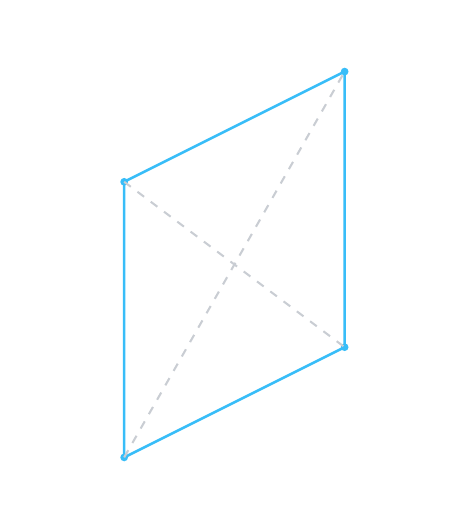
\begin{tikzpicture}[scale=0.7]
  \coordinate (A) at (0,0);
  \coordinate (B) at (0,5);
  \coordinate (C) at (4,7);
  \coordinate (D) at (4,2);

  \draw[seg] (A)--(B)--(C)--(D)--cycle;

  \fill[cyan] (A) circle (2pt);
  \fill[cyan] (B) circle (2pt);
  \fill[cyan] (C) circle (2pt);
  \fill[cyan] (D) circle (2pt);

  \node[ptlab, below left] at (A) {$A(0,0)$};
  \node[ptlab, left] at (B) {$B(0,5)$};
  \node[ptlab, above right] at (C) {$C(4,7)$};
  \node[ptlab, right] at (D) {$D(4,2)$};

  \draw[dseg] (A)--(C);
  \draw[dseg] (B)--(D);
\end{tikzpicture}
\end{center}
\end{QAPair}

% ============================================================
% Q3
% ============================================================

\begin{QAPair}{Question 3}
\textcolor{gold}{\bfseries Question:} Show that the four points $(5,8)$, $(7,5)$, $(3,5)$ and $(5,2)$ are the vertices of a rhombus.\par
\tcblower
\textcolor{green}{\bfseries Answer:}\par
Let
\[
A(5,8),\quad B(7,5),\quad C(5,2),\quad D(3,5),
\]
which forms the ``diamond'' in order $A\to B\to C\to D\to A$.

\[
\begin{aligned}
\Step{1}\;& AB=\sqrt{(7-5)^2+(5-8)^2}=\sqrt{2^2+(-3)^2}=\sqrt{13}.\\
\Step{2}\;& BC=\sqrt{(5-7)^2+(2-5)^2}=\sqrt{(-2)^2+(-3)^2}=\sqrt{13}.\\
\Step{3}\;& CD=\sqrt{(3-5)^2+(5-2)^2}=\sqrt{(-2)^2+3^2}=\sqrt{13}.\\
\Step{4}\;& DA=\sqrt{(5-3)^2+(8-5)^2}=\sqrt{2^2+3^2}=\sqrt{13}.\\
\Step{5}\;& AB=BC=CD=DA \Rightarrow \text{all four sides equal } \Rightarrow \text{rhombus.}
\end{aligned}
\]
\par\medskip
\begin{center}
\begin{tikzpicture}[scale=0.8]
  \coordinate (A) at (0,3);
  \coordinate (B) at (2,1);
  \coordinate (C) at (0,-1);
  \coordinate (D) at (-2,1);

  \draw[seg] (A)--(B)--(C)--(D)--cycle;

  \fill[cyan] (A) circle (2pt);
  \fill[cyan] (B) circle (2pt);
  \fill[cyan] (C) circle (2pt);
  \fill[cyan] (D) circle (2pt);

  \node[ptlab, above] at (A) {$(5,8)$};
  \node[ptlab, right] at (B) {$(7,5)$};
  \node[ptlab, below] at (C) {$(5,2)$};
  \node[ptlab, left] at (D) {$(3,5)$};

  \draw[dseg] (A)--(C);
  \draw[dseg] (B)--(D);
\end{tikzpicture}
\end{center}
\end{QAPair}

% ============================================================
% Q4
% ============================================================

\begin{QAPair}{Question 4}
\textcolor{gold}{\bfseries Question:} $A(3,4)$, $B(-1,7)$ and $C(x,y)$ are three collinear points such that $B$ is midpoint of $\overline{AC}$. Find values of $x$ and $y$.\par
\tcblower
\textcolor{green}{\bfseries Answer:}\par
\[
\begin{aligned}
\Step{1}\;& \text{Since }B\text{ is midpoint of }AC:\\
&\left(\frac{3+x}{2},\frac{4+y}{2}\right)=(-1,7).\\[4pt]
\Step{2}\;& \frac{3+x}{2}=-1 \Rightarrow 3+x=-2 \Rightarrow x=-5.\\
\Step{3}\;& \frac{4+y}{2}=7 \Rightarrow 4+y=14 \Rightarrow y=10.\\[4pt]
\Step{4}\;& \boxed{\,x=-5,\ y=10\,}\ \text{ so } C(-5,10).
\end{aligned}
\]
\end{QAPair}

\end{document}
